\chapter{\ifenglish Background Knowledge and Theory\else ทฤษฎีที่เกี่ยวข้อง\fi}
\tolerance = 9999
\overfullrule=0pt

% การทำโครงงาน เริ่มต้นด้วยการศึกษาค้นคว้า ทฤษฎีที่เกี่ยวข้อง หรือ งานวิจัย/โครงงาน ที่เคยมีผู้นำเสนอไว้แล้ว ซึ่งเนื้อหาในบทนี้ก็จะเกี่ยวกับการอธิบายถึงสิ่งที่เกี่ยวข้องกับโครงงาน เพื่อให้ผู้อ่านเข้าใจเนื้อหาในบทถัดๆ ไปได้ง่ายขึ้น
\enskip \enskip \enskip ในการตรวจสอบประกาศนียบัตรออนไลน์ด้วยบล็อคเชนก่อนที่จะลงมือสร้างนั้นผู้พัฒนาจำเป็นที่จะต้องไปศึกษาเกี่ยวกับ Blockchain ก่อนสำหรับสร้างซึ่งจะไปศึกษาจาก Hyperledger Fabric และใช้ Blockchain แบบ private
โดยเนื้อหาในบทนี้จะอธิบายในส่วนของความรู้ ทฤษฎีบทที่เกี่ยวข้อง และหลักการต่างๆที่ผู้พัฒนาได้ศึกษา และนำไปใช้ในการสร้าง Blockchain  
เพื่อให้ผู้ที่เข้ามาอ่านได้เข้าใจหลักการต่างๆในเบื้องต้น และเพื่อให้เข้าใจเนื้อหาในบทถัดๆไปได้ง่ายมากยิ่งขึ้น

\section{พื้นฐาน Blockchain}
\enskip \enskip \enskip \enskip \enskip 
\enskip \enskip 
\subsection{Blockchain คืออะไร}
Blockchain คือเทคโนโลยีว่าด้วยระบบการเก็บข้อมูล Data Structure ซึ่งไม่มีตัวกลาง แต่ข้อมูลที่ได้รับการปกป้องจะถูกแชร์และจัดเก็บเป็นสำเนาไว้ในเครื่องของทุกคนที่ใช้ฐานข้อมูลเดียวกันเสมือนห่วงโซ่ Chain โดยทุกคนจะรับทราบร่วมกัน ว่าใครเป็นเจ้าของและมีสิทธิในข้อมูลตัวจริง เมื่อมีการอัปเดตข้อมูลใด ๆ สำเนาข้อมูลในฐานเดียวกันก็จะอัปเดตตามไปด้วยทันที ทำให้การปลอมแปลงข้อมูลไม่ใช่เรื่องง่าย เพราะทุกคนต้องรับทราบและตรวจสอบความถูกต้องของข้อมูลร่วมกันได้ อีกทั้งไม่มีระบบล่ม และภัยใด ๆ ก็ไม่อาจทำลายอุปกรณ์ในระบบได้พร้อมกัน เช่นเดียวกับการถูกแฮ็กข้อมูล ซึ่งต้องทำการแฮ็กทุกเครื่องในฐานเดียวกันพร้อม ๆ กัน หรืออย่างน้อยต้องแฮ็กเครื่องที่ถือสำเนาให้ได้มากกว่าร้อยละ 51 จึงจะแฮ็กได้สำเร็จ เทคโนโลยี Blockchain จึงนับว่ายอดเยี่ยมในแง่ของเครดิตและความปลอดภัย นอกจากนี้ ยังเป็นเทคโนโลยีที่เข้ามารองรับการซื้อขายสกุลเงินดิจิทัล เช่น บิทคอยน์ Bitcoin ฯลฯ ให้มีความปลอดภัยด้านข้อมูลมากยิ่งขึ้นด้วย
\subsection{Blockchain แตกต่างจาก Database ทั่วๆไปอย่างไร}
คือ Blockchain จะมีการเก็บข้อมูลไว้เป็นกลุ่มๆ ไว้ใน block ซึ่งมัดรวมข้อมูลไว้ด้วยกัน ซึ่งมีการเก็บข้อมูลจะในมาต่อกับ block ก่อนหน้ามีลักษณะเป็นโซ่ ซึ่งถ้าข้อมูลก่อนหน้าผิดพลาดหรือถูกแก้ไขจะทำให้รู้ได้เพราะเหมือนโซ่ที่ขาดออกจากกัน แต่ในส่วนของdatabase ทั่วๆไปจะเก็บในรูปแบบของตารางซึ่งถ้าถูกแก้ไขจะทำให้เราไม่รู้ตัวได้ว่าถูกแก้ไขเมื่่อใด แต่ถ้า Blockchain  
\subsection{Public blockchain คือ}
คือ เป็น Blockchain ที่ทุกคนสามารถเข้าถึงและมีส่วนร่วมได้ เนื่องจากเป็น Open Network ทั้งหมด โดยลักษณะของการใช้งานพื้นฐานของ Blockchain ประเภทนี้ คือ การแลกเปลี่ยน Cryptocurrency และการขุด รวมถึงความสามารถในการรักษาความไว้วางใจระหว่าง Community ของผู้ใช้ทั้งหมด 
เนื่องจากทุกคนในเครือข่ายรู้สึกมีแรงจูงใจที่จะทำงานเพื่อพัฒนาเครือข่าย แต่ข้อเสียของ Blockchain ประเภทนี้ คือ ต้องใช้พลังงานจำนวนมากในการประมวลผลธุรกรรมเพราะใช้ระบบ Proof of work ในการตรวจสอบธุรกรรม และปัญหาอีกอย่างที่พบเจอคือ การเปิดกว้างเกินไป จึงทำให้ไม่มีความเป็นส่วนตัวในการทำธุรกรรมเท่าไรนัก
ตัวอย่างของ Public blockchain network เช่น Bitcoin  , Ethereum , BNB Chain ซึ่งต่างเป็น Blockchain ยอดนิยมที่ทุกคนสามารถเข้าถึงได้ง่าย
\subsection{Private blockchain คือ}
คือ Blockchain ที่ทำงานในเครือข่ายแบบปิด ซึ่งสามารถเข้าร่วมได้เฉพาะบุคคลที่ได้รับอนุญาตหรือคำเชิญเท่านั้น โดย Blockchain ประเภทนี้เหมาะที่สุดสำหรับองค์กรและธุรกิจที่ต้องการใช้ Blockchain สำหรับการใช้งานภายใน 
ขณะที่การทำธุรกรรมใน Private blockchain นั้นเร็วและง่ายเมื่อเทียบกับ Public blockchain แต่ข้อเสีย คือ ไม่มีการกระจายอำนาจ เนื่องจากมีผู้มีอำนาจเพียงคนเดียวที่ดูแลเครือข่าย
\subsection{ข้อดีของ Blockchain}
คือ ช่วยเพิ่มความปลอดภัยของข้อมูลและสามารถรู้ได้ว่าข้อมูลของเราถูกแก้ไขหรือดัดแปลงไหม

\section{พื้นฐาน Hyperledger Fabric}
\enskip \enskip \enskip \enskip \enskip Hyperledger Fabric เป็น private blockchain ซึ่งหมายความว่า ใครก็ตามที่ต้องการเข้าร่วมและใช้งานข้อมูลบน chain ในระบบ จะต้องได้รับสิทธิ์ก่อน จึงสามารถมองเห็นและใช้งานข้อมูลที่อยู่ใน chain นั้นๆได้ ซึ่งจะแตกต่างจาก public blockchain ที่ไม่ว่าจะเป็นใครก็สามารถมีสิทธิ์เข้าถึงข้อมูลบน ledger ได้นั่นเอง

Hyperledger Fabric เป็น Distributed Ledger ถูกออกแบบมาเพื่อใช้งานเกี่ยวกับการทำ transaction ระหว่างองค์กร โดยแต่ละองค์กรจะมีช่องทางที่ใช้สำหรับ communicate ซึ่งกันและกัน โดยที่องค์กรหนึ่งๆสามารถอยู่ได้หลายช่องทาง และแต่ละช่องทางนั้นข้อมูลจะถูกแยกจากกันอย่างชัดเจน

ด้วยพื้นฐานของโครงการที่ต้องการให้ Architecture ของ Hyperledger Fabric มีลักษณะเป็น Modular ตัว Hyperledger Fabric จึงประกอบด้วย Component สำคัญๆดังต่อไปนี้
\subsection{Peers}
 โดยส่วนตัวหากจะให้จินตนาการว่า Peers คืออะไร ก็ให้นึกถึง Network แบบ Peer-to-Peer โดย Peer ในที่นี้ก็คือ Node แต่ละ Node ภายใต้ Network ของ Blockchain นั้นๆ นั่นเอง

 \begin{figure}[htbp]
   \centering 
   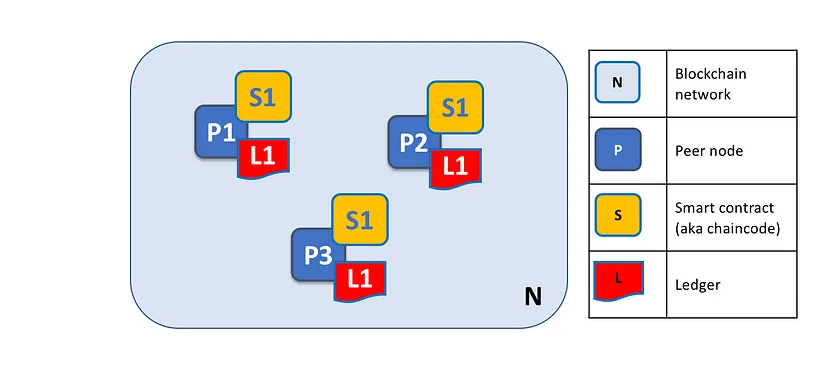
\includegraphics[scale=0.3]{peer.png}
   \caption[Peer]{ตัวอย่างของpeer
   ที่มา: https://hyperledger-fabric.readthedocs.io/en/release-2.2/peers/peers.html}
   \label{fig:Peer}
 \end{figure}



\subsection{Certificate Authorities}
หากพูดถึง Blockchain ก็ต้องบอกว่ามันเป็นกลุ่มของ Network ที่ทำหน้าที่ประมวลผลข้อมูลร่วมกัน โดยเฉพาะใน Permissioned Blockchain อย่าง Hyperledger Fabric ที่เราจำเป็นต้องรู้ว่าคนที่เข้ามาเป็นใคร ตัวจริงหรือไม่ มีสิทธิ์ในการเข้าถึง Network ในรูปแบบใดบ้าง

\begin{figure}[htbp]
  \centering 
  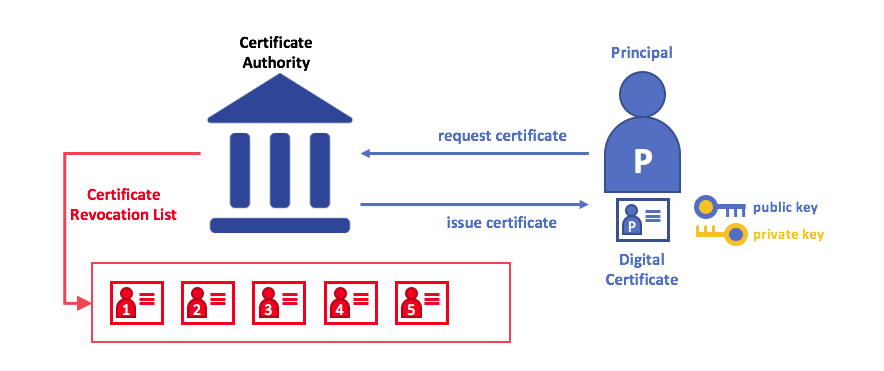
\includegraphics[scale=0.3]{certifi.png}
  \caption[Certificate Authorities]{Certificate Authorities
  ที่มา:https://hyperledger-fabric.readthedocs.io/en/release-2.2/peers/peers.html}
  \label{fig:Certificate}
\end{figure}

Certificate Authorities มีหน้าที่ Generate Identity ของทุกๆ Actor ที่ต้องการใช้งาน Network ของ Blockchain โดย Certificate Authorities จะสร้าง Digital Certificate ที่ระบุตัวตนของ Actor ตามมาตรฐาน X.509

\subsection{Ordering services}
ในโลกของ Hyperledger Fabric Ordering Service จะทำหน้าที่หลักๆ 2 ส่วน คือ
\begin{enumerate}
  \item Pack ตัว Transaction ที่ต้องการแก้ไข Ledger ที่ส่งเข้ามาจาก Application แต่ละตัว 
  \item กระจาย Pack ของ Transactionที่สร้างขึ้นนั้น ไปยังแต่ละ Peer ที่อยู่ใน Network
\end{enumerate}

โดยในแต่ละ Transaction ของการจัดการกับข้อมูลที่อยู่ใน Ledger จะประกอบไปด้วย 3 ระยะ คือ

\begin{enumerate}
  \item Proposal
  เป็นระยะที่เกิดขึ้นหลังจากที่ Application ปลายทางส่ง Request เข้ายัง Endorser เพื่อสร้าง Proposal สำหรับ Update ข้อมูล ขั้นตอนนี้เสร็จสิ้น Endorser จะส่ง Response กลับไปที่ Application
  \item Proposal
  เป็นระยะที่เกิดขึ้นหลังจากที่ Application ปลายทางส่ง Request เข้ายัง Endorser เพื่อสร้าง Proposal สำหรับ Update ข้อมูล ขั้นตอนนี้เสร็จสิ้น Endorser จะส่ง Response กลับไปที่ Application
  \item Validation and commit
  เมื่อ Peers ได้รับข้อมูล Transaction จาก Ordering Services หากข้อมูลมีความถูกต้องก็จะ Commit เข้าไปใน Ledger ของตัวเอง
\end{enumerate}

\subsection{Channels}
หากจะเปรียบเทียบว่า Channel ใน Hyperledger Fabric คืออะไร ก็ให้นึกถึงช่องทางที่เปิดให้เข้าถึงในแต่ละ Peer ของ Network นั้นๆ

\begin{figure}[htbp]
  \centering 
  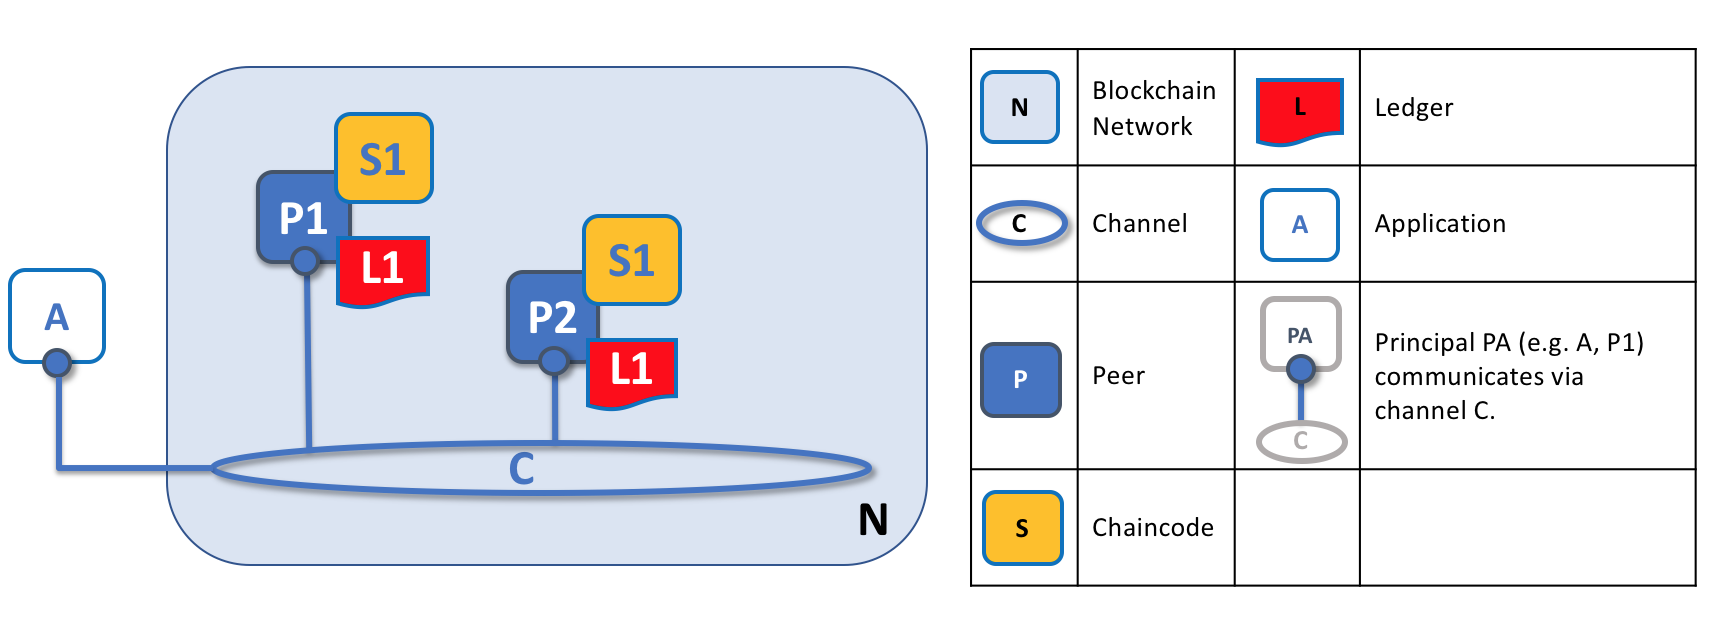
\includegraphics[scale=0.3]{peers diagram 5.png}
  \caption[peers diagram 5]{peers diagram 5
  ที่มา:https://hyperledger-fabric.readthedocs.io/en/release-2.2/peers/peers.html}
  \label{fig:peers diagram 5}
\end{figure}

ยกตัวอย่างในรูป การจะเข้าที่ Peer P1 และ P2 ได้ ก็จำเป็นที่จะต้องเข้าผ่าน Channel C ที่ถูกสร้างขึ้น แต่ถ้าหากใน Network นี้มี Peer P3 อยู่ในภายใน Network Application A ก็จะไม่สามารถเข้าถึงได้ เนื่องจาก Channel C ที่ถูกสร้างขึ้น ไม่ได้เชื่อมต่อกับ Peer P3 ที่ถูกสร้างขึ้นนั้นเอง

\subsection{Chaincode หรือ Smart Contracts}
หากใครใช้งาน Eterium ก็คงจะรู้จัก Smart Contract ที่เขียนด้วย Solidity ของ Eterium มาบ้างเช่นกัน โดย Concept อาจจะไม่ต่างกัน โดย Chaincode จะมีลักษณะเหมือนโปรแกรมขนาดเล็ก ที่เปิดให้ Application ส่งคำสั่งเข้ามาประมวลผลข้อมูลที่อยู่ภายใน Ledger ได้ สำหรับ Hyperledger Fabric เปิดให้นักพัฒนาสามารถพัฒนา Chaincode ผ่านทาง Fabric SDK ได้ด้วยภาษาที่ค่อนข้างหลากหลาย ได้แก่ Go, Javascript หรือ Java

\section{การเขียนโปรแกรมเชิงวัตถุ(Object Oriented Programming : OOP)}
\enskip \enskip \enskip \enskip \enskip การเขียนโปรแกรมเชิงวัตถุ เป็นการเขียนโปรแกรมประเภทหนึ่ง โดยใช้แนวคิดในการพัฒนา software 
ที่มอง code เป็นวัตถุ(object)แทนการเขียน code เป็น streaming ต่อกันยาวๆ การเขียนโปรแกรมเชิงวัตถุ
ช่วยทำให้ Developer เห็นภาพรวมของ code ได้ง่ายขึ้น สามารถทำความเข้าใจ และแก้ไขข้อผิดพลาดต่างๆได้ถูกจุดอย่างรวดเร็ว 
เพราะการเขียน code แบบโปรแกรมเชิงวัตถุ code จะถูกแบ่งเป็นส่วนๆ(class)อย่างชัดเจน ซึ่งช่วยให้หา code ได้ง่ายขึ้น  
นอกจากนั้น หลักการการเขียนโปรแกรมเชิงวัตถุไม่ได้ยึดติดกับภาษาในการเขียนภาษาใดภาษาหนึ่ง ดังนั้นการเขียนโปรแกรมเชิงวัตถุ หรือ OOP จึงออกแบบมาเพื่อให้ code
ที่เราเขียนมีแบบแผน เหมาะสมในการพัฒนา software ที่ซับซ้อน ซึ่งในการสร้างเกมก็ต้องใช้หลัการของ OOP ในการเขียน code เพื่อใช้ในการควบคุมการทำงานต่างๆภายในเกม 
หรือที่เรียกว่า script

\enskip \enskip \enskip \enskip \enskip ในการเขียนโปรแกรมเชิงวัตถุ เราจะเทียบ code กับวัตถุในชีวิตจริง เช่น มนุษย์(player) ซึ่งจะให้ player เป็นวัตถุ 
โดยสิ่งที่ player ต้องมีก็คือ คุณสมบัติ(Attribute) เช่น ผู้ชาย, สูง, ผมสั้น เป็นต้น และต้องมี พฤติกรรม(Behavior) เช่น เดิน, วิ่ง, กระโดด เป็นต้น 
การเขียนโปรแกรมก็ต้องทำให้ code ของเรามีคุณสมบัติและพฤติกรรมเช่นเดียวกันกับ player ซึ่งทำได้โดยการสร้าง class ของ player ขึ้นมา โดยใน class ที่สร้าง
นั้นจะมีทั้ง Attribute และ Behavior ของ player ดังที่กล่าวมา และเมื่อจะนำ class ไปใช้งาน จะทำได้โดยการสร้าง object ขึ้นมา เปรียบเสมือนเป็น player หนึ่งคน
โดย player ที่สร้างมานั้น จะมีทั้ง Attribute และ Behavior เหมือนของ class player ดังกล่าว


\enskip \enskip \enskip \enskip \enskip สำหรับการเขียนโปรแกรมเชิงวัตถุ หรือ OOP ประกอบไปด้วยหลักการที่สำคัญอยู่ 4 ข้อ ได้แก่ 

\begin{enumerate}
\item Encapsulation คือ การห่อหุ้มข้อมูล หรือการซ่อนข้อมูล สามารถทำได้โดยการกำหนดสถานะของ สิ่งที่ไม่อยากให้ใครเข้าถึง หรือแก้ไขได้ ให้มีสถานะ
เป็น private กล่าวคือ เรามาสามารถกำหนดสถานะให้กับ Attribute และ Behavior ภายใน class ต่างๆให้เป็น private ได้ ซึ่งจะทำให้ class ภายนอก หรือผู้ใช้ ไม่สามารถเข้ามา
แก้ไขข้อมูลนั้นๆได้ ช่วยแก้ไขเหตุการณ์ที่เมื่อเรามีหลาย object ที่มาจากหลายๆ class เมื่อไม่ได้กำหนดสถานะเป็น private จะทำให้ทุกๆ object สามารถเข้าไปแก้ไข เปลี่ยนแปลง Attribute 
และ Behavior ของ object ตัวอื่นๆได้อย่างอิสระ ซึ่งอาจจะทำให้เกิดความผิดพลาดในการทำงานได้ถ้าถูกเปลี่ยนแปลงคุณสมบัติโดยไม่มีการควบคุม  
\item Abstraction คือ การทำให้ผู้ใช้หรือ ภายนอกรู้เท่าที่จำเป็น ซึ่ง Abstraction เป็นผลพลอยได้จาก Encapsulation เพราะเป็นการเลือกเปิดแค่บบางสิ่งในบาง object ให้คนอื่นเห็น หรือกล่าวได้ว่า
object ภายนอกสามารถเรียกใช้ Attribute หรือ Behavior ของ object ตัวที่เปิดให้เข้าถึงได้ โดยที่ object ที่มาใช้งานไม่รู้ว่าการทำงานเบื้องหลังทำอย่างไรบ้าง แต่รู้แค่ว่า ใช้ในทำอะไร
\item Inheritance คือ การทำเรามี class ที่จะสร้างขึ้นมาใหม่ แต่ class ใหม่นั้นมีความใกล้เคียงกับ class เก่าที่มีอยู่เเล้ว แต่ไม่ใช่ตัวเดียวกัน หากเราสร้าง class ใหม่โดยสร้าง Attribute และ Behavior ขึ้นมาเองใหม่หมด
จะทำให้เปิดความสิ้นเปลือง ดังนั้น Inheritance จึงมาช่วยแก้ไขในส่วนนี้ โดยการที่ class ใหม่ที่เราสร้าง จะสามารถนำ Attribute และ Behavior ของ class เก่ามาใช้ได้โดยไม่ต้องสร้างขึ้นมาใหม่ และสามารถแก้ไข เพื่มลดการทำงานได้ 
โดยจะเรียกการแก้ไขแบบนี้ว่า การ Overdrive 
\item Polymorphism คือ การที่เรามีหลายๆ class ที่คล้ายๆกัน และอยากให้แต่ละ class เหล่านั้นมี Attribute และ Behavior ที่เรียกใช้งานในทุกๆ class ให้ได้เหมือนๆกัน
จึงใช้ Polymorphism มาช่วยแก้ไขปัญหาเหล่านี้ โดยการสร้าง class ต้นแบบที่มี Attribute และ Behavior ที่เราต้องการเตรียมไว้ และให้ class ที่คล้ายๆกันดังกล่าว เข้ามาสืบทอดไปสร้างการทำงาน
ของตัวเองเอง เช่น class หมากับ class แมว มี Behavior การเกิดเหมือนกัน เมื่อเราใช้ Polymorphism เราก็สร้างการทำงานของการเดินของแต่ละ class ได้ ซึ่งอาจจะเดินไม่เหมือนกัน แต่เราจะเรียกใช้
 Behavior ได้ในลักษณะที่คล้ายกัน กล่าวคคือ Behavior มีชื่อเดียวกัน ทำหน้าที่เดียวกัน แต่อาจจะมีขึ้นตอนการทำงานคนละแบบกัน
\end{enumerate}

\section{Vector}
\enskip \enskip \enskip \enskip \enskip ปริมาณทางคณิตศาสตร์มีสองแบบ คือ scalar เป็นปริมาณที่อธิบายด้วยปริมาณขนาด(magnitude)เพียงอย่างเดียว และ vector เป็นปริมาณที่อธิบายด้วยขนาด(magnitude) และทิศทาง(direction)
ปริมาณทาง vector ถูกใช้ในหลากหลายศาสตร์ ไม่ว่าจะเป็น คณิตศาสตร์ ฟิสิกส์ เคมี และอื่นๆ ตัวอย่างปริมาณทาง vector เช่น ความเร็ว การกระจัด
การเคลื่อนที่ต่างๆ แรง สนามแม่เหล็ก เป็นต้น ซึ่งในการสร้างเกม 3D ขึ้นมา ปริมาณทาง vector มีความสำคัญอย่างมาก เนื่องจากต้องใช้ในการคำนวณ ทิศทาง ตำแหน่งของ GameObject และใช้ในการทำให้ GameObject เกิดการ
เคลื่อนที่ กล่าวคือ การสร้างเกม 3D ก็เหมือนการจำลองสร้างสภาพแวดล้อมให้เหมือนของจริง มีความเร็ว มีแรง มีมวล ซึ่งต้องอาศัยความรู้ทางปริมาณทาง Vector
\enskip \enskip \enskip โดยความรู้ทางปริมาณทาง vector ที่ต้องใช้คือ
\begin{enumerate}
\item การเขียน vector โดย vector ประกอบไปด้วย 3 ส่วนคือ vector ในทิศทางแกน x y z ซึ่งจะนำมาเขียนในรูปแบบทางคณิตศาสตร์ได้โดยใช้ วงเล็บ เช่น (1,2,-4) ซึ่งก็คือ vector ที่ประกอบ
ไปด้วย vector ตามแกน x ที่มีขนาด 1 หน่วย vector ตามแกน y ที่มีขนาด 2 หน่วย และ vector ตามแกน z ที่มีขนาด -4 หน่วย
\item Magnitude vector คือ การหาขนาดของ vector โดยขนาดของ vector จะเป็นปริมาณทาง scalar ซึ่งใช้ในการคำนวณขนาดต่างๆได้ โดยสามารถหาขนาดของ vector ได้จาก
สูตร vector V = (x, y, z) มีขนาดเท่ากับ $$ |\vec{V}| = \sqrt{x^2 + y^2 + z^2} $$ โดยสัญลักษณ์ขนาดของ vector V ใดๆแทนด้วย $ |\vec{V}| $
\item Normalize vector คือ การทำให้ vector ที่เรามี มีขนาดเป็น 1 หน่วย หรือเรียกว่า vector 1 หน่วย โดยสามารถทำได้จากการทำ Normalization ซึ่งก็คือ การนำขนาดของ vector มาก
หารกับ vector ตัวนั้นๆ ดังนี้ $$ \hat{V} = \frac{\vec{V}}{|\vec{V}|} $$ 
เมื่อ $ \vec{V} $ คือ vector ใดๆ และ $ \hat{V} $ คือ vector 1 หน่วยของ $ \vec{V} $
\item Distance คือ การหาระยะหว่างระหว่าง vector 2 ตัวใดๆ ซึ่งเป็นปริมาณทาง scalar นำมาประยุกต์ใช้ในการคำนวณตำแหน่งต่างๆ, หาแรงที่ต้องใช้ได้ ซึ่งหาระยะทางได้จากสูตร
$$ D_{UV} = \sqrt{(u_x - v_x)^2 + (u_y - v_y)^2 + (u_z - v_z)^2}  $$
เมื่อ $ D_{UV} $ คือ ระยะห่างระหว่าง $ \vec{U} $, $ \vec{V} $ และ $ \vec{U} = (u_x, u_y, u_z)$,  $ \vec{V} = (v_x, v_y, v_z) $
% \begin{equation} Unit(V) = \frac{V}{||V||} \end{equation}
\end{enumerate}

\section{ระบบพิกัดคาร์ทีเซียนสามมิติ (Cartesian coordinate system)}
\enskip \enskip \enskip \enskip \enskip เป็นระบบที่ใช้กำหนดตำแหน่งของจุดแต่ละจุดบนพิกัดฉาก โดยอ้างถึงตัวเลข 3 จำนวน 
ซึ่งแต่ละจำนวนเรียกว่า พิกัด x พิกัด y และพิกัด z ของจุดนั้นๆ และเพื่อที่จะกำหนดพิกัดของจุดใดๆ จะต้องมีเส้นแกนสามเส้นตัดกันเป็นมุมฉากที่จุดกำเนิด
ได้แก่ แกน x แกน y และแกน z ซึ่งเส้นแกนดังกล่าวจะมีหน่วยบ่งบอกความยาวเป็นระยะ ระบบพิกัดคาร์ทีเซียนสามมิติยังสามารถใช้ได้ในปริภูมิสองมิติ 
หรือในมิติที่สูงกว่าได้ ตัวอย่างเช่น จุด a อยู่ที่พิกัด x = 3 พิกัด y = 5 พิกัด z = 4 หรือเขียนเป็น (3, 5, 4) 
\graphicspath{ {./images/} }

\begin{figure}[htbp]
  \centering 
  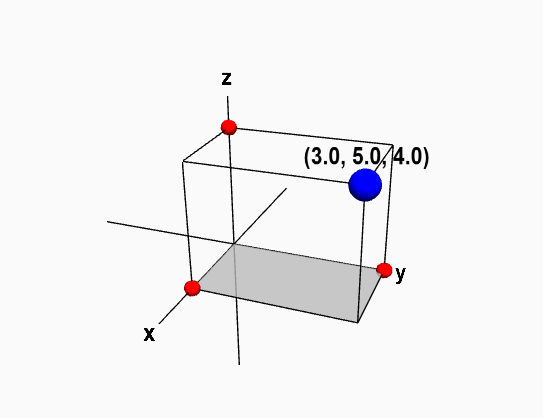
\includegraphics[scale=0.5]{cartesian coordinate 3d.png}
  \caption[Cartesian coordinate]{ตัวอย่างจุดบนระบบพิกัดคาร์ทีเซียนสามมิติ}
  \label{fig:cartesian}
\end{figure}
ซึ่งในการสร้างเกมเราจำเป็นต้องระบุตำแหน่งต่างๆของ GameObject ดังนั้นการสร้างเกมใน Unity จึงจำเป็นต้องรู้จักกับระบบพิกัดคาร์ทีเซียนสามมิติด้วย


\section{State Machine}
\enskip \enskip \enskip \enskip \enskip คือ การทำงานแบบมีการเปลี่ยนสถานะการทำงาน(state)ไปเรื่อยๆ เป็นขั้นตอนๆอย่างชัดเจน ซึ่งเป็นการมองสถานะการทำงานต่างๆ
เป็น state โดยที่เมื่อ input เข้ามาก็จะมีการเปลี่ยนสถานะการทำงาน(เปลี่ยนไป state ใหม่) หรืออาจจะไม่เปลี่ยนก็(อยู่ที่ state เดิม)ได้ขึ้นกับ input ซึ่งการจะเปลี่ยนสถานะแต่ละครั้ง
ขึ้นกับหลายๆอย่าง ได้แก่สถานะปัจจุบัน input เงือนไขต่างๆที่มีผลต่อการเปลี่ยนสถานะ ตัวอย่าง state machine เช่น ระบบประตูอัตโนมัติ โดยจะมีอยู่สอง state คือ ปิด และเปิด 
โดยเมื่อถ้าประอยู่ state "ปิด" แล้วมี input คือ มีคนอยู่หน้าประตู หลังจากได้รับ input ประตูก็จะเปลี่ยน state ไปเป็น "เปิด" ซึ่งถ้าไม่มีคนเเล้วประตูก็จะเปลี่ยน state เป็น "ปิด"
ซึ่งในการสร้างเกมมีการนำ state machine เข้ามาใช้ในการแสดง animation ต่างๆ ไม่ว่าจะเป็น การเดิน การวิ่ง การกระโดด โจมตี และอื่นๆ
% \begin{center}
% 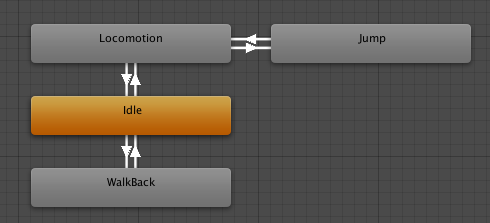
\includegraphics[scale=0.6]{MecanimStateMachine.png}
% \end{center}
% \begin{center}
% รูปที่ 2.2: ตัวอย่าง State Machine ที่ใช้ควบคุม animation
% \end{center}
% \graphicspath{ {./images/} }

\begin{figure}[htbp]
  \centering 
  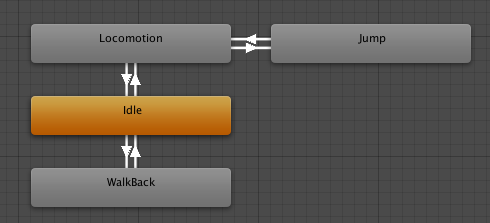
\includegraphics[scale=0.6]{MecanimStateMachine.png}
  \caption[State Machine]{ตัวอย่าง State Machine ที่ใช้ควบคุม animation}
  \label{fig:stateMachine}
\end{figure}

\section{ภาษา \texttt{C\#}}
\enskip \enskip \enskip \enskip \enskip เป็นภาษาคอมพิวเตอร์ที่เขียนโปรแกรมแบบ multi-paradigm~\cite{multiParadigm} โดยมีรูปแบบกฎเกณฑ์ และ
ข้อบังคับในการเขียนที่เข้มงวด ซึ่งมีคุณสมบัติในการเขียนแบบ function เหมือนกับการเขียนภาษาทั่วไป และเป็นการเขียนโปรแกรมแบบ OOP โดย \texttt{C\#} ถูกพัฒนาโดย 
Microsoft ภายใต้ .NET Framework~\cite{NET_Framework} โดยในการพัฒนาภาษา \texttt{C\#} นี้ มีความตั้งใจให้เป็นภาษาที่เขียนง่าย ทันสมัย 

\enskip \enskip \enskip ใน Unity ภาษา \texttt{C\#} ถูกนำมาใช้เป็นภาษาหลักในการเขียน script หรือ code ที่ทำหน้าที่จัดการกับการทำงานต่างๆในเกม
โดยรองรับหลากหลาย Framework เช่น Visual studio, VS code เป็นต้น

% \subsubsection{Subsubsection 1 heading goes here}
% Subsubsection 1 text

% \subsubsection{Subsubsection 2 heading goes here}
% Subsubsection 2 text

% \section{Third section}
% Section 3 text. The dielectric constant\index{dielectric constant}
% at the air-metal interface determines
% the resonance shift\index{resonance shift} as absorption or capture occurs
% is shown in Equation~\eqref{eq:dielectric}:

% \begin{equation}\label{eq:dielectric}
% k_1=\frac{\omega}{c({1/\varepsilon_m + 1/\varepsilon_i})^{1/2}}=k_2=\frac{\omega
% \sin(\theta)\varepsilon_\mathit{air}^{1/2}}{c}
% \end{equation}

% \noindent
% where $\omega$ is the frequency of the plasmon, $c$ is the speed of
% light, $\varepsilon_m$ is the dielectric constant of the metal,
% $\varepsilon_i$ is the dielectric constant of neighboring insulator,
% and $\varepsilon_\mathit{air}$ is the dielectric constant of air.

% \section{About using figures in your report}

% define a command that produces some filler text, the lorem ipsum.
% \newcommand{\loremipsum}{
%   \textit{Lorem ipsum dolor sit amet, consectetur adipisicing elit, sed do
%   eiusmod tempor incididunt ut labore et dolore magna aliqua. Ut enim ad
%   minim veniam, quis nostrud exercitation ullamco laboris nisi ut
%   aliquip ex ea commodo consequat. Duis aute irure dolor in
%   reprehenderit in voluptate velit esse cillum dolore eu fugiat nulla
%   pariatur. Excepteur sint occaecat cupidatat non proident, sunt in
%   culpa qui officia deserunt mollit anim id est laborum.}\par}

% \begin{figure}
%   \centering

%   \fbox{
%      \parbox{.6\textwidth}{\loremipsum}
%   }

%   % To include an image in the figure, say myimage.pdf, you could use
%   % the following code. Look up the documentation for the package
%   % graphicx for more information.
%   % \includegraphics[width=\textwidth]{myimage}

%   \caption[Sample figure]{This figure is a sample containing \gls{lorem ipsum},
%   showing you how you can include figures and glossary in your report.
%   You can specify a shorter caption that will appear in the List of Figures.}
%   \label{fig:sample-figure}
% \end{figure}

% Using \verb.\label. and \verb.\ref. commands allows us to refer to
% figures easily. If we can refer to Figures
% \ref{fig:walrus} and \ref{fig:sample-figure} by name in the {\LaTeX}
% source code, then we will not need to update the code that refers to it
% even if the placement or ordering of the figures changes.

% \loremipsum\loremipsum

% % This code demonstrates how to get a landscape table or figure. It
% % uses the package lscape to turn everything but the page number into
% % landscape orientation. Everything should be included within an
% % \afterpage{ .... } to avoid causing a page break too early.
% \afterpage{
%   \begin{landscape}
%   \begin{table}
%     \caption{Sample landscape table}
%     \label{tab:sample-table}

%     \centering

%     \begin{tabular}{c||c|c}
%         Year & A & B \\
%         \hline\hline
%         1989 & 12 & 23 \\
%         1990 & 4 & 9 \\
%         1991 & 3 & 6 \\
%     \end{tabular}
%   \end{table}
%   \end{landscape}
% }

% \loremipsum\loremipsum\loremipsum

% \section{Overfull hbox}

% When the \verb.semifinal. option is passed to the \verb.cpecmu. document class,
% any line that is longer than the line width, i.e., an overfull hbox, will be
% highlighted with a black solid rule:
% \begin{center}
% \begin{minipage}{2em}
% juxtaposition
% \end{minipage}
% \end{center}

\section{\ifenglish%
\ifcpe CPE \else ISNE \fi knowledge used, applied, or integrated in this project
\else%
ความรู้ตามหลักสูตรซึ่งถูกนำมาใช้หรือบูรณาการในโครงงาน
\fi
}
\enskip \enskip \enskip \enskip \enskip ในการทำโครงงานนี้กลุ่มของพวกเราได้นำความรู้ตามหลักสูตรต่างๆ มาประยุกต์ใช้ ซึ่งได้แก่
\subsection{ความรู้ที่ได้จากหลักสูตรวิชา Object Oriented Programming 261200}
\begin{enumerate}
\item การเขียนโปรแกรมเชิงวัตถุ(Object Oriented Programming : OOP) โดยการเขียนโปรแกรมเชิงวัตถุ กลุ่มของพวกเราได้นำมาใช้ในการวางแผน โดยการสร้าง interface และเขียน script ควบคุมการทำงาน โดยจะมีการออกแบบระบบต่างๆในเกมเป็น class 
เช่น class ของ characterController ใช้ควบคุมการควบคุมตัวละครโดยรวม, Status ใช้ในการควบคุมสถานะต่างๆของตัวละคร, AttackPoint ใช้คำนวณ damage จากการต่อสู้ เป็นต้น 
\item การนำเอา design patterns มาใช้ในการเขียน code โดยในส่วนที่ต้องการให้ object ใดๆมีเพียงแค่ตัวเดียวได้มีการนำ Singleton มาใช้ เพื่อป้องการทำงานซ้ำซ้อนของ code, ในส่วน
ที่เป็นการคำนวณ damage ซึ่งการ damage มีอยู่หลากหลายรูปแบบ เช่น damage จากการโจมตีเเบบ 1 hit, damage จากการโจมตีเเบบต่อเนื่อง(ติดสถานะต่างๆ), damage จากการโจมตี magic attack เป็นต้น
ซึ่งเพื่อให้ code มีความยืดหยุ่นเมื่อมีการโจมตีรูปแบบใหม่เพิ่มเข้ามา จึงได้มีการใช้ Strategy เข้ามาช่วย ซึ่งจะทำการสร้าง interface รวมที่คอยจัดการเกี่ยวกับการคำนวณ damage ต่างๆไว้ที่เดียวกัน นอกจากนี้ยังมี
code ส่วนอื่นๆก็มีการนำ design patterns มาใช้เช่นกัน
\end{enumerate}

\subsection{ความรู้ที่ได้จากหลักสูตรวิชา Calculus III 206261}
\begin{enumerate}
\item การคำนวณทางปริมาณ vector โดยได้นำความรู้ต่างๆในเรื่อง calculus vector มาใช่ในการคำนวณต่างๆภายในเกม เช่น ทิศทางการเดิน, ทิศทางการโจมตี เป็นต้น 
รวมถึงการนำความรู้ทาง vector มาช่วยในการทำความเข้าใจการทำงานต่างๆของ method ต่างที่อยู่ใน Unity
\item ความเร็ว ความเร่ง โดยได้นำความรู้เรื่อง อัตราการเปลี่ยนแปลงของความเร็ว คือ ความเร่ง มาประยุกต์ใช้ในการหาความเร็วของวัตถุ
\end{enumerate}

\subsection{ความรู้ที่ได้จากหลักสูตรวิชา Data Structure 261217}
\enskip \enskip \enskip การเก็บข้อมูลในรูปแบบต่างๆ โดยใน Unity การเขียน script บางครั้งต้องมีการเก็บข้อมูลต่างๆในเกมที่มีลักษณะที่แตกต่างกันออกไป ซึ่งข้อมูลเหล่านี้
จะเหมาะกับการเก็บใน structure ต่างๆแตกต่างกันออกไป เช่น การเก็บของที่ตัวละครเก็บได้ ควรจะเก็บเป็นรูปแบบ key และ value โดย key เป็น ชื่อของสิ่งของ
ส่วน value คือ จำนวนของสิ่งของนั้นๆ เป็นต้น

\subsection{ความรู้ที่ได้จากหลักสูตรวิชา ฟิสิกส์ 1 207105}
\begin{enumerate}
\item ปริมาณทางฟิสิกส์ โดยในการสร้างเกม ระบบของเกมจะอิงตามหลักความเป็นจริง ซึ่งได้มีการใช้ปริมาณทางฟิสิกส์ต่างๆ เช่น ความเร็ว, ความเร่ง, 
แรงเสียดทาน, แรงโน้มถ่วง, มวล เป็นต้น
\item การเคลื่อนที่ต่างๆ มีการเคลื่อนที่หลากหลายรูปแบบที่สามารถเกิดขึ้นภายในเกมได้ เช่น การเคลื่อนที่ในแนวดิ่ง, การเคลื่อนที่วิถีโค้ง(projectile), การเคลื่อนที่แบบมีแรงเสียดทานต่างๆ เป็นต้น
\end{enumerate}

\subsection{ความรู้ที่ได้จากหลักสูตรวิชา discrete mathematics 261216}
\begin{enumerate}
\item state machine โดยใช้ในการควบคุมการทำงานของ animation ของตัวละครต่างๆภาายในเกม
\item ความรู้ทางด้านตรรกศาสตร์ ใช้ในการออกแบบ เงื่อนไขต่างๆภายในเกม
\end{enumerate}



% อธิบายถึงความรู้ และแนวทางการนำความรู้ต่างๆ ที่ได้เรียนตามหลักสูตร ซึ่งถูกนำมาใช้ในโครงงาน

\section{\ifenglish%
Extracurricular knowledge used, applied, or integrated in this project
\else%
ความรู้นอกหลักสูตรซึ่งถูกนำมาใช้หรือบูรณาการในโครงงาน
\fi
}
\enskip \enskip \enskip \enskip \enskip ในการทำโครงงานนี้กลุ่มของพวกเราได้นำความรู้นอกหลักสูตรต่างๆ มาประยุกต์ใช้ ซึ่งได้แก่

\subsection{ความรู้ทางด้านการสร้างเกมโดยใช้ Unity}
\enskip \enskip \enskip เนื่องจากเกมของกลุ่มพวกเราใช้ Unity ในการพัฒนา ดังนั้นจึงได้มีการศึกษาการใช้งาน function ส่วนประกอบต่างๆใน
Unity ดังที่กล่าวไว้ในข้อ 2.1 พื้นฐาน Unity และได้มีการไปศึกษาในส่วนของ VFX หรือ Visual effect เพื่อนำมาปรับใช้กับตัวเกมหลัก  

\subsection{ความรู้ทางด้านการเขียนภาษา \texttt{C\#}}
\enskip \enskip \enskip เนื่องจากเกมของกลุ่มพวกเราใช้ Unity ในการพัฒนา ซึ่งใช้ภาษา \texttt{C\#} ในการเขียน script กลุ่มของพวกเราจึงได้ทำการศึกษาเพิ่มเติมกันเอง
โดยอาศัยสื่อต่างๆทางอินเตอร์เน็ต เช่น youtube, unimy, google เป็นต้น ดังที่กล่าวไว้ในข้อ 2.7 ภาษา \texttt{C\#}

\subsection{ความรู้ทางด้านการปั้น Model โดยใช้ Blender}
\enskip \enskip \enskip เนื่องจากมาจากมี asset บางอย่างที่จำเป็นต้องมีในเกม แต่ asset เหล่านั่นไม่สามารถหาซื้อได้ หรือมีราคาแพงจนเกินไป หรือไม่มีขาย 
จึงจำเป็นที่จะต้องปั้น Model ขึ้นมาใช้เอง เช่น ถังน้ำ, ก้อนหิน, บันได เป็นต้น

\enskip \enskip \enskip และในบางครั้ง Model ที่ซื้อมามี shader ที่ไม่ต้องการ หรืออยากปรับ shader ให้เป็นรูปแบบที่ต้องการ จึงต้องใช้ Blender ช่วยในการ
จัดการกับประเด็นเหล่านี้ ดังที่กล่าวไว้ในข้อ 2.2 พื้นฐาน Blender



% อธิบายถึงความรู้ต่างๆ ที่เรียนรู้ด้วยตนเอง และแนวทางการนำความรู้เหล่านั้นมาใช้ในโครงงาน
